\chapter{Behaviorism}\label{chapter:behaviorism}

The player forms the root of Gamification and, in any system, the outcome is affected and driven by his motivation (Zichermann \& Cunningham, 2011, p. 15). Therefore, to understand the potentials and fundamental aspects behind Gamification, one important part is to understand what drives people's motivation. Thus, psychology is  essential  to  Gamification  in order to understand  how  human  nature  works  and  how  it can  be  influenced  in  order  to  create  an  effective  Gamified  system. For this reason, the next sections introduce different views from psychology about motivation and explain what has to be considered in terms of truly engaging individuals. There are two main purposes of this section. The first is to provide a suitable overview of the subject itself and to introduce terms that will be used later in the discussion. The second purpose is to present theories that describe and explain various psychological effects that games have on players.

\subsection{The Rules of Motivation}

The word \textit{motivation} originates from Latin \textit{motivus} and stands for ``serve to move''. In other words, motivation can be interpreted as \textit{to be moved to do something}. It can be defined as ``those forces within an individual that push or propel him to satisfy basic needs or wants'' \cite{pardee1990motivation}. One of the most influential researchers in the domain of human motivation and behavior, Richard M. Ryan \& Edward L. Deci (2010b), argue that people \textit{can be moved} to act by various types of factors, as so with highly diverse experiences and consequences. For example, people can be motivated because they value the activity they perform, or because there exists some external influence and pressure. Furthermore, they point out that each person has different amounts and also different kinds of motivation. That is, each person is different in level (i.e. how much motivation) and orientation (i.e. what type of motivation) of their motivation, whereas orientation might be a goal which give rise to action and therefore governs human behavior.  % A motive is what prompts the person to act in a certain way, or at least develop an inclination for specific behavior. 
According to Zichermann \& Cunningham, there exist four underlying reasons why people are motivated to play games, which can be viewed together or separately as individual motivators (Zichermann \& Cunningham, 2011, p. 20). These reasons are as follows:
\begin{itemize}
\item For mastery
\item To destress
\item To have fun
\item To socialize
\end{itemize} 

People play games not so much for the game itself as for the experience
that the game creates: an exciting adrenaline rush, a vicarious adventure, a mental challenge;
and the structure games provide for time, such as a moment of solitude or the company of
friends.
Nicole Lazzaro, an expert on player experience and emotions in games, 

%%TODO: OVO MOZDA NA KRAJU....

SDT
\section{Self Determination Theory}
%deci ima dva papera
Another aspect to understanding player motivations is by questioning the source of one's motivation. One of the most influential motivational theories is the Self Determination Theory (SDT) introduced by Ryan \& Deci. It is an empirically derived theory of human motivation that makes distinctions between different types of motivation in terms of reasons and goals that cause the respective action. That is, SDT proposes that behaviors that are intentional might vary in the extent to which they are \textit{self-determined} versus \textit{controlled}. This means that behaviors can vary in the extent they are experienced as being freely chosen and coming from one's self in contrary to being pressured or controlled externally. When these behaviors are experienced as freely chosen they are considered self-determined or autonomous, whereas the extent they are experienced as coerced, they are considered controlled \cite{deci1994promoting}. Having this in mind, SDT distinguishes between \textit{Intrinsic} and \textit{Extrinsic}motivation. The first type of motivation, as the word \textit{intrinsic} already suggests, refers to performing an activity for the inherent satisfaction. When intrinsically motivated, a person is moved to act because the activity is challenging, interesting and enjoyable on its own rather than because of some external prods, pressures, or rewards. On the other hand, extrinsic motivation refers to performing an action because it leads to \textit{separable outcome}. That is, there is some external reward or influence which drives the person to accomplish the task (Deci  \& Ryan, 2000). The comparison between people intrinsically and those extrinsically motivated (TOCHECK) reveals that the former have more interest, excitement, and confidence which in turn, can not only enhance performance, persistence, and creativity but consequently boost vitality, increase self-esteem and general well-being \cite{ryan2000self}. Though this division is for most people intuitively understandable, it is not always as clear as it may seem. For example, as the SDT theory states, \textit{motivations are fluid}. Hence, people can convert extrinsic motivators to intrinsic if they internalize the desire to do so. To put it more simply, in a situation where the extrinsic motivator is found meaningful, pleasurable and consistent with a person’s worldview, it can be percieved and adopted as it was intrinsic \cite{zichermann2012}.
Although, in one sense, intrinsic motivation can exist within an individual, in another sense, it can exist in the relation between the individual and the activity one performs. Having that in mind, it is important to point out that not everyone is intrinsically motivated for the same activities and that not everyone is intrinsically motivated for any particular activity \cite{ryan2000intrinsic}. In SDT, the \textit{basic psychological need satisfaction} is assumed to be the core motivational mechanism that directs human's behavior. SDT postulates three innate psychological needs, that are ``essential for ongoing psychological growth, integrity, and well-being'' and all three of them play a necessary part in optimal development, hence none can be disregarded without significant negative consequences. These needs are the need for autonomy, competence and relatedness and when individuals experience them, they become self-determined and intrinsically motivated to pursue thing the interest them \cite{deci2000and}. %https://selfdeterminationtheory.org/SDT/documents/2010_VandenBroeckVansteenkisteNSscale_JOOP.pdf
\begin{itemize}
\item \textbf{Autonomy} represents individuals' innate desire to feel \textit{free} and to experience a sense of choice and psychological freedom when carrying out certain activities \cite{deci2000and}. Situations in which individuals are provided with the opportunity to choose freely, accompanied with a positive feedback, have been shown to influence and improve autonomy and, hence, the intrinsic motivation of individuals [ryan 2006]. For example, students  are  autonomous when they willingly spend time and energy to completing their assignments. 
\item \textbf{Competence} represents individuals' innate desire to feel effective when interacting with the environment. For example, students are competent in cases they feel they can meet the challenges of their schoolwork. Furthermore, Deci \& Ryan (2000) point out that positive feedback can signify effectance and provide a satisfaction of the need for competence, thus enhancing intrinsic motivation, whereas negative feedback that convey ineffectance, tend  to
diminish the sense of competence and hence undermine intrinsic motivation. 

%A. P. Hill, "A Brief Guide to Self-Determination Theory," September 2011. [Online]. Available: http://www.heacademy.ac.uk/assets/hlst/documents/projects/round_11/r11_hill_guide.pdf. [Accessed 10 April 2013].

\item \textbf{Relatedness} corresponds to experiencing meaningful connection to others,that is, to be a member of a group, to love and care and to be loved and cared for \cite{broeck2010capturing}. This psychological need is satisfied when individuals experience a sense of togetherness and develop a close and intimate relationship with others. 
\end{itemize}

The specification of autonomy, competence, and relatedness is important because it allows the prediction of variables that can affect individual's intrinsic motivation and the development of their extrinsic motivation \cite{deci1994promoting}. These needs can be achieved by means of diverse game elements, which will be discussed in detail in the next section.\\*\\*
Despite the observable evidence that humans, in general, can have intrinsic motivational tendencies towards some activities, this bias appears to manifest only in certain conditions and circumstances. Hence, SDT also places much emphasis on understanding conditions that enhance and sustain versus subdue and diminish intrinsic motivation.  A sub-theory of SDT called Cognitive evaluation  theory (CET) was presented by Deci and Ryan (1985) focuses on social and environmental factors that promote or undermine this type of motivation using language that reflects the assumption that intrinsic motivation, as an inherent bias, is rather catalyzed than caused when individuals are in appropriate socio-enviromental circumstances(Ryan  and  Deci  2000;  Ryan and Deci 2000b). In other words, intrinsic motivation does not occur by itself, but represents the outcome of one's interaction with the environment and one's interests and preferences. That is, intrinsic motivation ``will flourish if circumstances permit'' \cite{ryan2000self}. Furthermore, CET, which focuses mainly on the fundamental needs for competence and autonomy, argues that interpersonal events and structures, such as rewards, communication or feedback can increase intrinsic motivation for certain action because they satisfy the basic psychological need for competence. Accordingly, it is predicted that optimal challenges positive feedback and freedom from degrading evaluations promote intrinsic motivation while tangible rewards, threats,  deadlines  and  directives  decrease it(Ryan \& Deci, 2000). Furthermore, CET also argues that the satisfaction of the psychological needs for competence will not enhance intrinsic motivation unless they are joined by a sense of autonomy. Hence, people must perceive that their behavior is self-determined in order for intrinsic motivation to be maintained or enhanced. In other words, for a high level of intrinsic motivation, the needs for competence and autonomy must both be satisfied (Ryan \& Deci, 2000). It is important to point out, as stated by Ryan \& Deci, (2000) that people will be intrinsically motivated for certain activities only when they are intrinsically captivating for an individual, that means activities that offer a degree of novelty, challenge or aesthetic value. Activities that do not provide such appeal, will not be experienced as intrinsically motivated. \\*\\*
Even though intrinsic motivation is of great importance, most of the activities people do are not intrinsically motivated. Such activities, being uninteresting and unsatisfactory for individuals  require external \textit{push} in order to be realized. This motivation, contrary to intrinsic motivation which refers to doing an activity simply for the enjoyment of the activity itself, is known as extrinsic motivation. It refers to performing certain activities because it is expected to result in some additional outcome or reward that have an instrumental value for the individual performing that action \cite{ryan2000self}. In general, extrinsically motivated behaviors are ones that would not happen instinctively, and hence must be prompted by an intrumentality \cite{deci1994promoting}. Various studies demonstrated that in specific circumstances extrinsic motivation can sustain intrinsic motivation, thus suggesting that extrinsically motivated behaviors can also be self-determined \cite{deci1994promoting}. Extrinsically motivated behaviors become self-determined through the process of \textit{internalization} and \cite{integration}. Internalization involves transforming internal regulatory processes into internal regulatory processes, while integration corresponds to the process of integrating these now internalized values and regulation into one's self \cite{deci1994promoting}. There exists four types of extrinsic regulation that can result from different types of internalization and integration, which were introduced within SDT as a subtheory called Organismic Integration Theory (OIT) \cite{ryan2000intrinsic, ryan2000self, deci1994promoting}. For instance, students who work on their assignments because they personally understand it's importance for their future career and those who do it only to adhere to their parents' control are both extrinsically motivated. Even though both cases involve instrumentalities rather than enjoyment, the former entails personal endorsement and a feeling of choice while the latter associates only with an external regulation.\\*
Figure \ref{fig:tax} illustrates the IOT taxonomy of motivational types arranged from left to right in terms of the degree to which the motivation originate from the self (i.e. are self-determined).\\*
\begin{figure}[h]
    \centering
    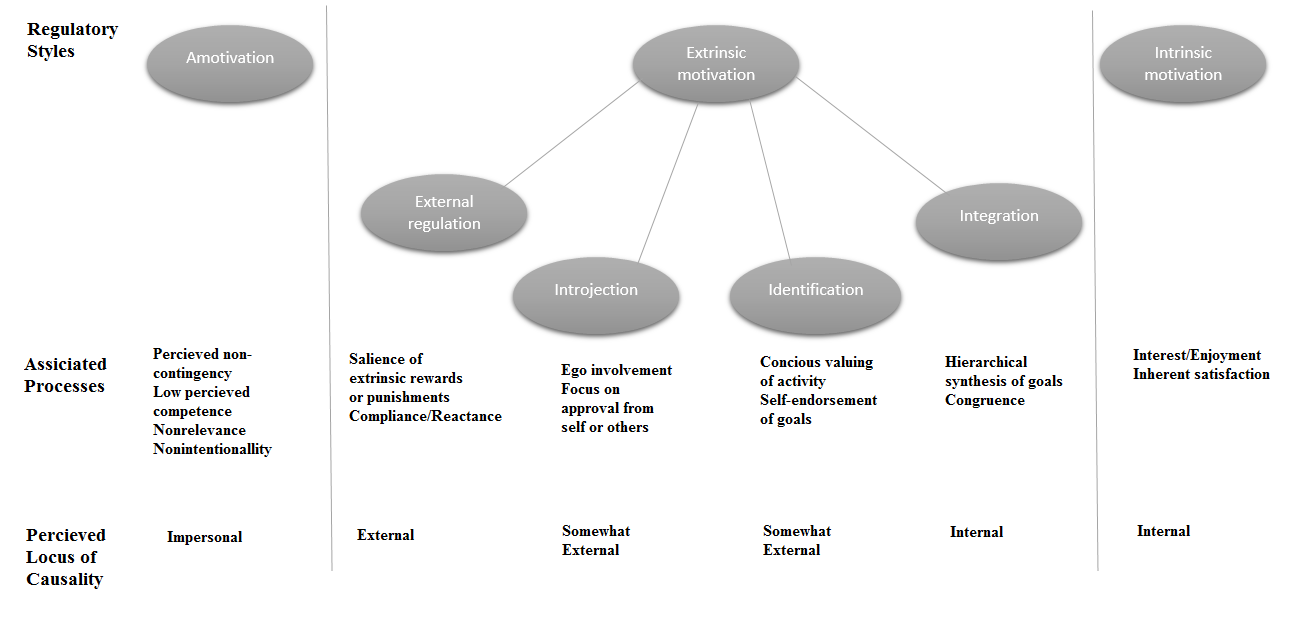
\includegraphics[width=\textwidth]{taxm}
    \caption{The Self-Determination Continuum showing types of Motivation}
    \label{fig:tax}
\end{figure}\\*
First, extrinsically motivated behavior that is the least autonomous is known as \textit{External Regulation} and is regulated through some external means, such as rewards and constraints. For example, an athlete who participates in the Olympics onlt to obtain a medal represesents an instance of externally regulated behavior. In case of \textit{Introjected regulation}, individuals begin to internalize the reasons for their action. However, this internalization only replaces the external source of motivation with an interalnal one, such as guilt, worry or shame. That is, when people are motivated to perform activity in order to maintain feeling of worth. An example for introjection is the athlete who goes to the practice just because he would feel guilty if it has been skipped. A more autonomous of extrinsic motivation, \textit{identification} manifests when a person is identified with the importance of some behavior and accepted it as a personal regulation only because it benefits the athlete in achieving a specific goal. An example for this behavior is a runner who does not like weight lifting, but nevertheless chooses to to do it because it will positively impact her future performance. \textit{Integrated regulation} as the most autonomous of extrinsic motivation that shares many qualities with intrinsic motivation is a form of motivation that arises when an individual has fully assimilated the identified regulation within himself. An example of integrated regulation is an athlete who chooses postpone the night out with his friend in order to be in good shape for the next day's tournament. Integration together with intrinsic motivation represent the core for self-determined functioning and they both share the qualities that constitutes self-determination. Even though they might seem quite similar, they are different in sense that intrinsically motivated behaviors are ``autotelic in nature'' while, on the other hand, integrated behaviors are ``instrumentally (though freely) performed'' for the outcome that is self satisfactory.  Finally, the self-determination continuum is closed with  \textit{amotivation} which represents ``non-regulation'' from the SDT perspective as it refers to a state where intentions to act are non existent. A person amotivated towards exercise would not exercise at all, 
or engage in exercise in a passive and disorganised  manner \cite{vallerand2007intrinsic, ryan2000intrinsic, deci1994promoting}.

\subsection{Motivation and Sports}

pelletier1995toward

Vallerand (2004) states that motivation in sports matters, as it ``represents one of the most important variables in sport''. It is known to be a key element of success in sport and athletes' persistence with an exercise regiment \cite{vallerand2007intrinsic}. Intrinsic and extrinsic motivation have been particularly popular topics that allowed researchers to explain various phenomena of importance in sport and physical activity. Various studies in the domains of health, physical education, exercise and sport have explored the SDT derived hypothesis that intrinsically relative to extrinsically motivated behavior  

... is this necessary? 
\subsection{Key elements}
Armed with a clear understanding of the theory behind human motivation, this section will shed light on game elements (mechanics/dynamics), player types and the theory of flow in context of Gamification. The goal of this section is to provide a brief overview of the most relevant key elements, based on the research done on motivational theory and Gamification literature.





\section{State of Flow}
so-called state of flow of Mihály Csíkszentmihályi plays an
important role in gamification and can be considered as one of the basic concepts. Csíkszentmihályi
was a professor for psychology at University of Chicago and taught business
management at Claremont Graduate University in California (Csíkszentmihályi, 1995)
(Claremont Graduate University, 2014). In an article in the Journal of Humanistic Psychology
he described in 1975 for the first time the phenomenon of flow (Csíkszentmihályi,
1995). A short time later, he published the book Beyond Boredom and Anxiety, which
addressed this issue in a more comprehensive form (Csíkszentmihályi, 1995).